\begin{figure}[t!]
        \centering
	\begin{subfigure}{3.5in}\vspace{-5pt}
		\centering
		\begin{tikzpicture}
		\node at (0,0) {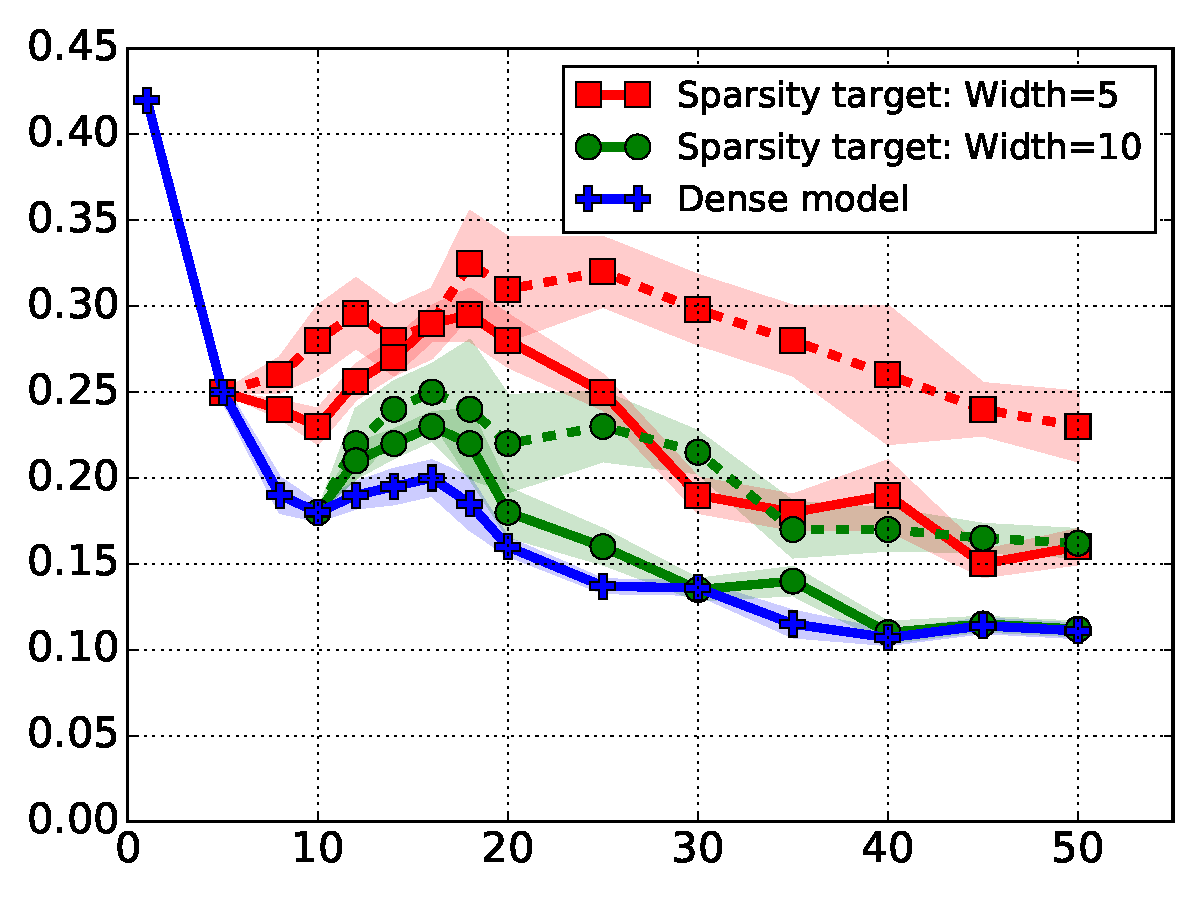
\includegraphics[scale=0.33]{figs/CIFAR10_random_DD}};
		\node at (-3.5,0) [rotate=90,scale=.9]{Test Error};
		\node at (0,-2.8) [scale=.9]{Width Parameter (\# of filters $k$)};%Each bar in the figure shows the correlations' geometric mean of datasets in this group when training to corresponding non-zero level. 
		\end{tikzpicture}\caption{\small{Magnitude-based and randomly pruned models.}}\label{figCFa}\vspace{-0.2cm}
	\end{subfigure}~~~~~\begin{subfigure}{3.5in}\vspace{-5pt}
	\centering
	\begin{tikzpicture}
	\node at (0,0) {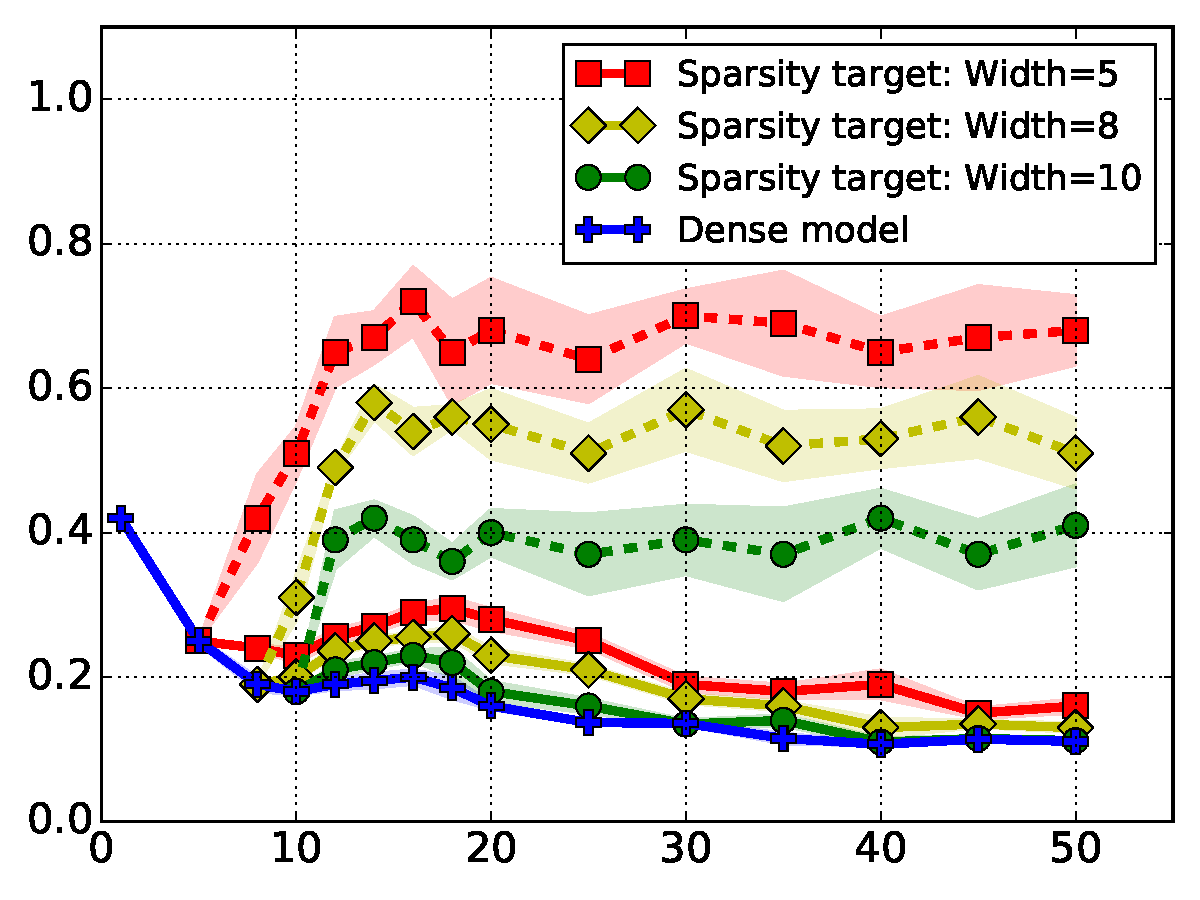
\includegraphics[scale=0.33]{figs/CIFAR10_without_retrain_DD}};
	%\node at (-2.4,0) [rotate=90,scale=1.]{Test Risk};
		\node at (-3.5,0) [rotate=90,scale=.9]{Test Error};
	\node at (0,-2.8) [scale=.9]{Width Parameter (\# of filters $k$)};%Each bar in the figure shows the correlations' geometric mean of datasets in this group when training to corresponding non-zero level. 
	\end{tikzpicture}\caption{\small{With and without retraining pruned models.}}\label{figCFb}\vspace{-0.2cm}
\end{subfigure}\caption{\small{We train and prune ResNet-20 models on CIFAR-10 and also add randomly pruning and non-retraining curves. Solid lines here are exactly the same as Figure \ref{figNN} which show test errors of dense and $s$-sparse models. Dotted lines are test errors of random-based pruned models in (a) and of magnitude-based pruned models however without retraining in (b).}}\label{figCF}\vspace{-10pt}
\end{figure}


\begin{figure}[t!]
        \centering
	\begin{subfigure}{1.8in}\vspace{-5pt}
		\centering
		\begin{tikzpicture}
		\node at (0,0) {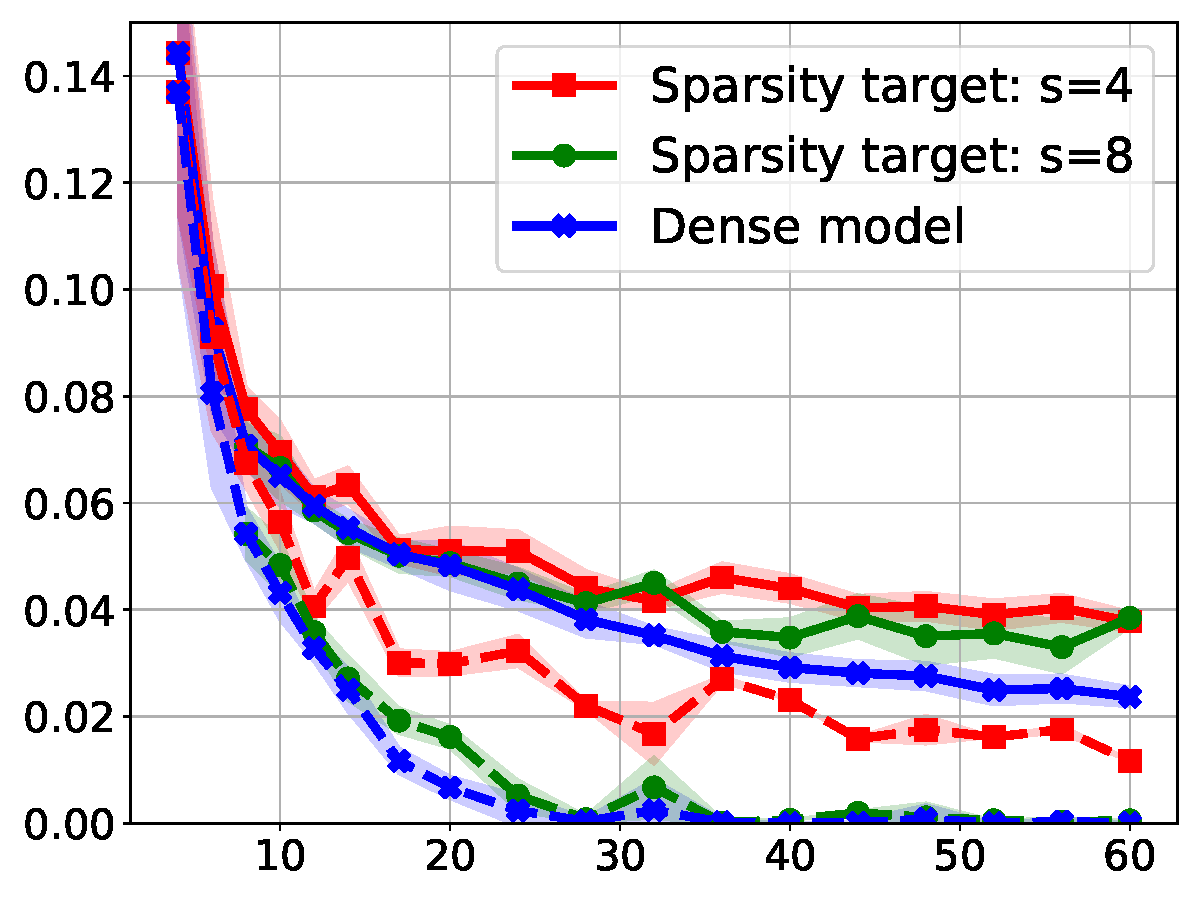
\includegraphics[scale=0.23]{figs/MNIST_MAGNITUDE}};
		\node at (-2.4,0) [rotate=90,scale=.9]{Training / Test Error};
		\node at (0,-1.9) [scale=.9]{Width Parameter (\# of nodes $k$)};%Each bar in the figure shows the correlations' geometric mean of datasets in this group when training to corresponding non-zero level. 
		\end{tikzpicture}\caption{\small{Dense and magnitude-based pruned and retrained models.}}\label{figMNISTa}\vspace{-0.2cm}
	\end{subfigure}~~~~~\begin{subfigure}{1.8in}\vspace{-5pt}
	\centering
	\begin{tikzpicture}
	\node at (0,0) {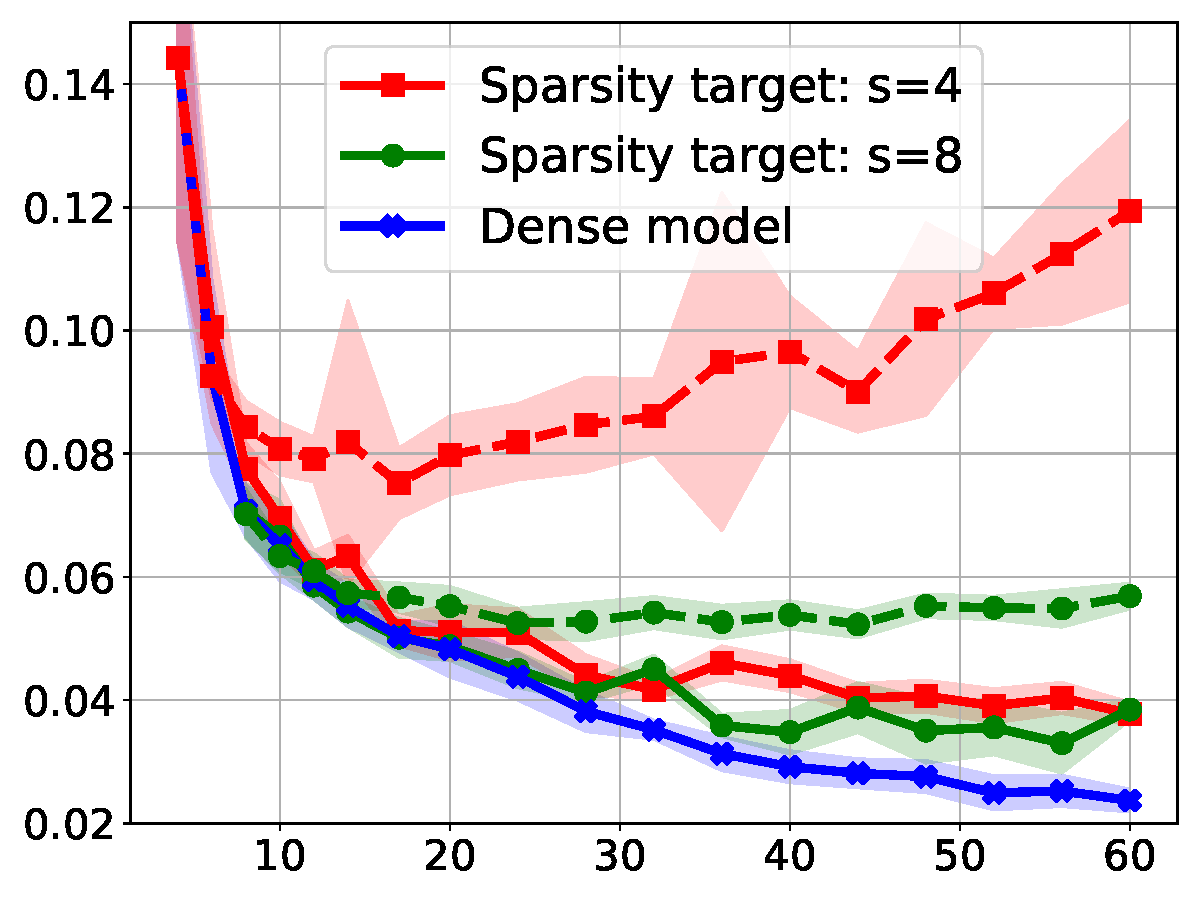
\includegraphics[scale=0.23]{figs/MNIST_RANDOM}};
	\node at (-2.4,0) [rotate=90,scale=.9]{Test Error};
	\node at (0,-1.9) [scale=.9]{Width Parameter (\# of nodes $k$)};%Each bar in the figure shows the correlations' geometric mean of datasets in this group when training to corresponding non-zero level. 
	\end{tikzpicture}\caption{\small{Magnitude-based and randomly pruned models.}}\label{figMNISTb}\vspace{-0.2cm}
\end{subfigure}~~~~~\begin{subfigure}{1.8in}\vspace{-5pt}
	\centering
	\begin{tikzpicture}
	\node at (0,0) {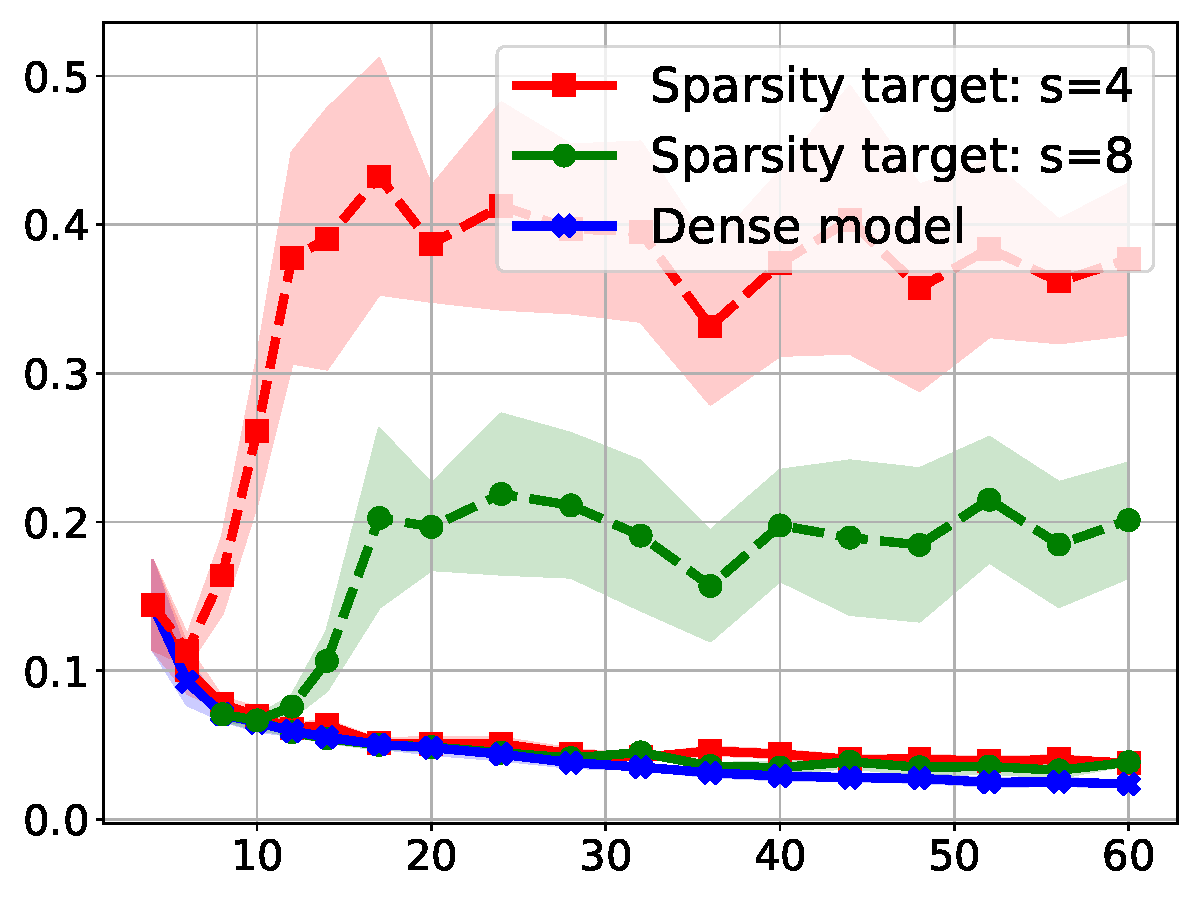
\includegraphics[scale=0.23]{figs/MNIST_NON_RETRAIN}};
	\node at (-2.4,0) [rotate=90,scale=.9]{Test Error};
	\node at (0,-1.9) [scale=.9]{Width Parameter (\# of nodes $k$)};%Each bar in the figure shows the correlations' geometric mean of datasets in this group when training to corresponding non-zero level. 
	\end{tikzpicture}\caption{\small{With and without retraining pruned models.}}\label{figMNISTc}\vspace{-0.2cm}
\end{subfigure}\caption{\small{Here we use the simplest neural network consisting of two fully-connected layers to train MNIST with various width and sparsity targets. In this architecture the width parameter equivalent to the number of hidden layer nodes controls model size. Same as Figure~\ref{figNN} the blue line corresponds to training dense models with width $k$. As for the red and green lines we choose $4$- and $8$-width models as base models respectively and prune $k$-width dense model to corresponding sparsity targets. (a) shows both training and test errors after magnitude-based pruning and retraining. In (b) solid and dotted lines are test errors of magnitude- and random-based pruned models with retraining. To verify the importance of retraining in neural networks we present the test errors of magnitude-based models without retraining in (c).}}\label{figMNIST}\vspace{-10pt}
\end{figure}


%
\section{Further Experiments and Intuitions}\label{SM mot}
%\newpage
%\newpage
% (Chang, Lizzie please fill here)
%\subsection{Verifying Analytical Predictions


%\subsection{Experiments on Neural Networks}
%\som{Explain retraining of Figure 1.}

\subsection{Further discussion and experiments on CIFAR-10} \label{ssec:SMCF}
First, we provide further discussion on Figure \ref{figNN}. Recall that, in this figure, we apply \emph{train$\rightarrow$prune$\rightarrow$retrain} to obtain the sparse neural networks. The test error and the training errors for the sparse models are evaluated at the end of the retraining phase. Thus, it is rather surprising that sparse models manage to achieve zero training error around the same width parameter $k$ as the dense model because while parameter count of the dense model increases in $k$, it is fixed for sparse models.

Secondly, we complement Figure \ref{figNN} with two additional experiments. The first experiment assesses the benefit of pruning compared to using a random nonzero pattern with the same sparsity. The second experiment assesses the benefit of retraining by comparing the curves in Fig \ref{figNN} with the test errors obtained without retraining. These two experiments are shown in Figure \ref{figCFa} and \ref{figCFb} and all of them are trained over same dataset and configured as given in Section \ref{ssec:NNE}. Instead of applying magnitude-based pruning, dotted red and green lines in Fig \ref{figCFa} are sparse models over $5$ or $10$ sparsity targets, pruned randomly to achieve same number of nonzeros as magnitude-based pruning strategy. Although the double descent phenomenon and downward trend are still present on the dotted lines, the performance is worse than magnitude-base pruning method. Fig. \ref{figCFb} shows how retraining benefits pruning ResNet-20 models. The results agree with our intuition that the non-retrained (dotted) lines achieve much bigger test error than retrained (solid) lines and overparameterization does not help in improving performance.

\subsection{MNIST Experiments with two layers} 
In Figure \ref{figMNIST} we train the simplest neural model with only 2 fully-connected layers over MNIST with various number of nodes to explore properties of magnitude-based pruning, random pruning and non-retraining on simple neural networks. Here, the number of nodes is equivalent to the width of the model, which directly controls the model size. Same as in Section \ref{ssec:NNE}, we select an $s$-width model as base model and prune trained dense models to the same sparsity. All experiments are trained with Adam optimization, $0.001$ learning rate and $200$ epochs under MNIST.  Solid red, green and blue lines in Figure \ref{figMNIST} correspond to test error of $4$-, $8$-sparsity targets and dense models. In Figure \ref{figMNISTa} dotted lines are training errors of dense and $s$-sparse models. As the width $k$ grows, the training and test error decrease for all dense and sparse models. The behavior is similar to Figure \ref{figNN} and training larger models benefit pruned-model accuracy however double descent is not really visible. We suspect that this may be because of the simpler nature of the MNIST dataset and LeNet architecture compared to the CIFAR10 dataset and ResNet-20 model. In Figure \ref{figMNISTb}, dotted lines apply randomly pruning. Different to magnitude pruning, where training bigger models and then pruning results in better performance, randomly pruning hurts when the sparsity level $s/k$ is relatively low. This is because under magnitude-based pruning, we can identity most of optimal entries of weights from trained dense model and retraining with these entries achieves lower errors. In constrast, random pruning learns nothing from the trained model and as the sparsity level decreases, the probability that random operator selects the limited optimal entries by chance also decreases, leading to worse performance. Dotted lines in Figure \ref{figMNISTc} show test errors of sparse models before retraining which educes the same conclusion in Section \ref{ssec:SMCF}, that is retraining is crucial to improve the performance in neural networks. 


\subsection{Experiments on LGP}
In Figure \ref{figSM1}, we carry out the identical experiments as in Figure \ref{fig1}. The difference is that we display two more figures which are the retraining curves for Magnitude- and Hessian-based pruning strategies shown in purple and yellow lines respectively. Figure \ref{figSM1a} is the counterpart of Figure \ref{fig1a} and Figure \ref{figSM1b} is the counterpart of Figure \ref{fig1b}. The main message in these experiments is that \emph{retraining hurts the performance}. This performance degradation is more emphasized in the overparameterized regime. Specifically, both retrained versions of Magnitude and Hessian pruning $\bth^{RT,M}$ and $\bth^{RT,H}$ perform consistently worse compared to their pruning-only counterparts $\bth^{M}$ and $\bth^{H}$. Observe that, the only regime where retraining outperforms the pruning-only approach is at the peak of double descent. This is the region where pruning-only risk diverges to infinity whereas retraining attains finite risk. This is because the retraining stage solves a well-conditioned problem and avoids the ill-conditioning occurring at $n=k$. Recall that, in light of Lemma \ref{lem rank one}, unlike the rank-one covariance case, retraining hurts because covariance is diagonal; thus, features are uncorrelated and do not have overlapping predictions.


\begin{figure}[t!]
        \centering
	\begin{subfigure}{3.5in}\vspace{-5pt}
		\centering
		\begin{tikzpicture}
		\node at (0,0) {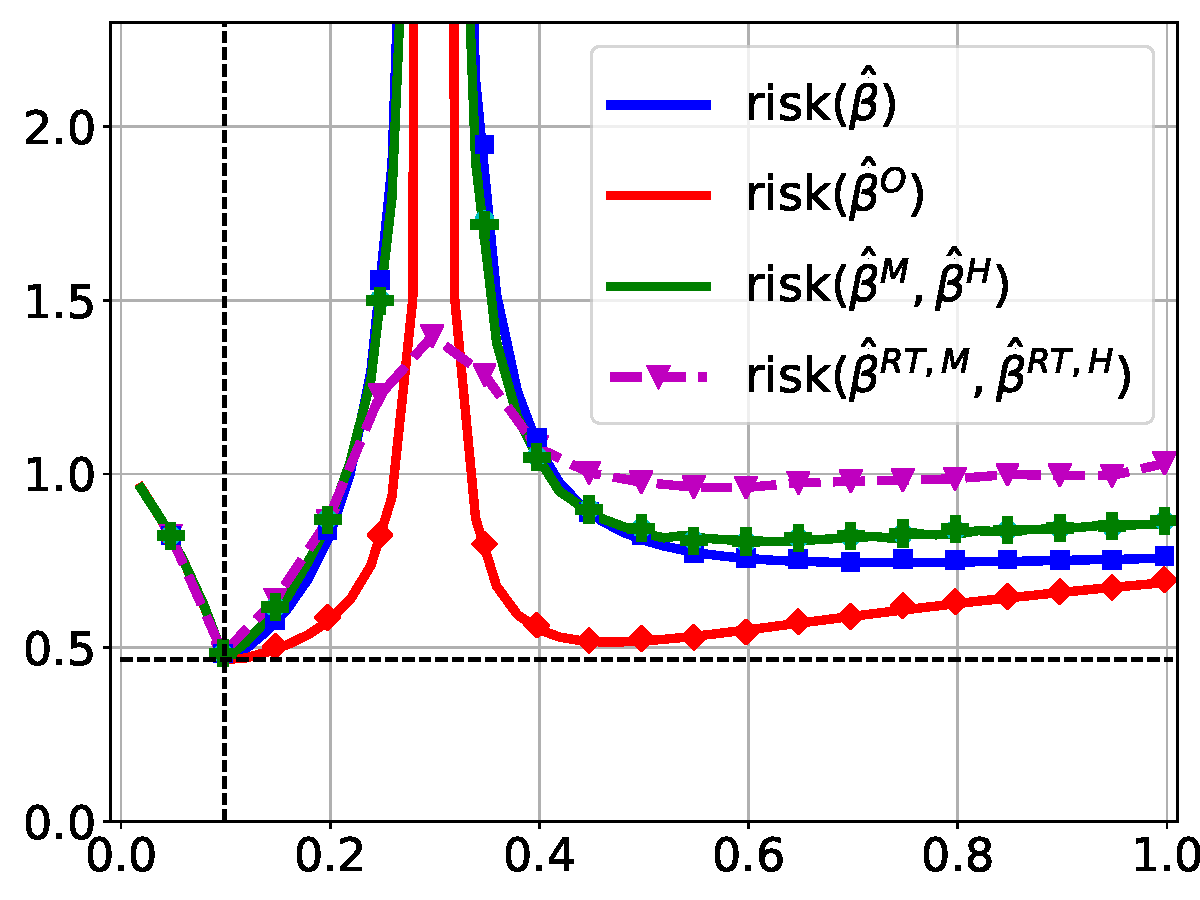
\includegraphics[scale=0.33]{figs/FLAT_SIM_RT_s10_n30_p100_SCL25}};
		\node at (-3.5,0) [rotate=90,scale=.9]{Test Risk};
		\node at (0,-2.8) [scale=.9]{Problem Size ($k/p$)};%Each bar in the figure shows the correlations' geometric mean of datasets in this group when training to corresponding non-zero level. 
		\end{tikzpicture}\caption{\small{Identity covariance, spiked latent weights.}}\label{figSM1a}\vspace{-0.2cm}
	\end{subfigure}~~~~~\begin{subfigure}{3.5in}\vspace{-5pt}
	\centering
	\begin{tikzpicture}
	\node at (0,0) {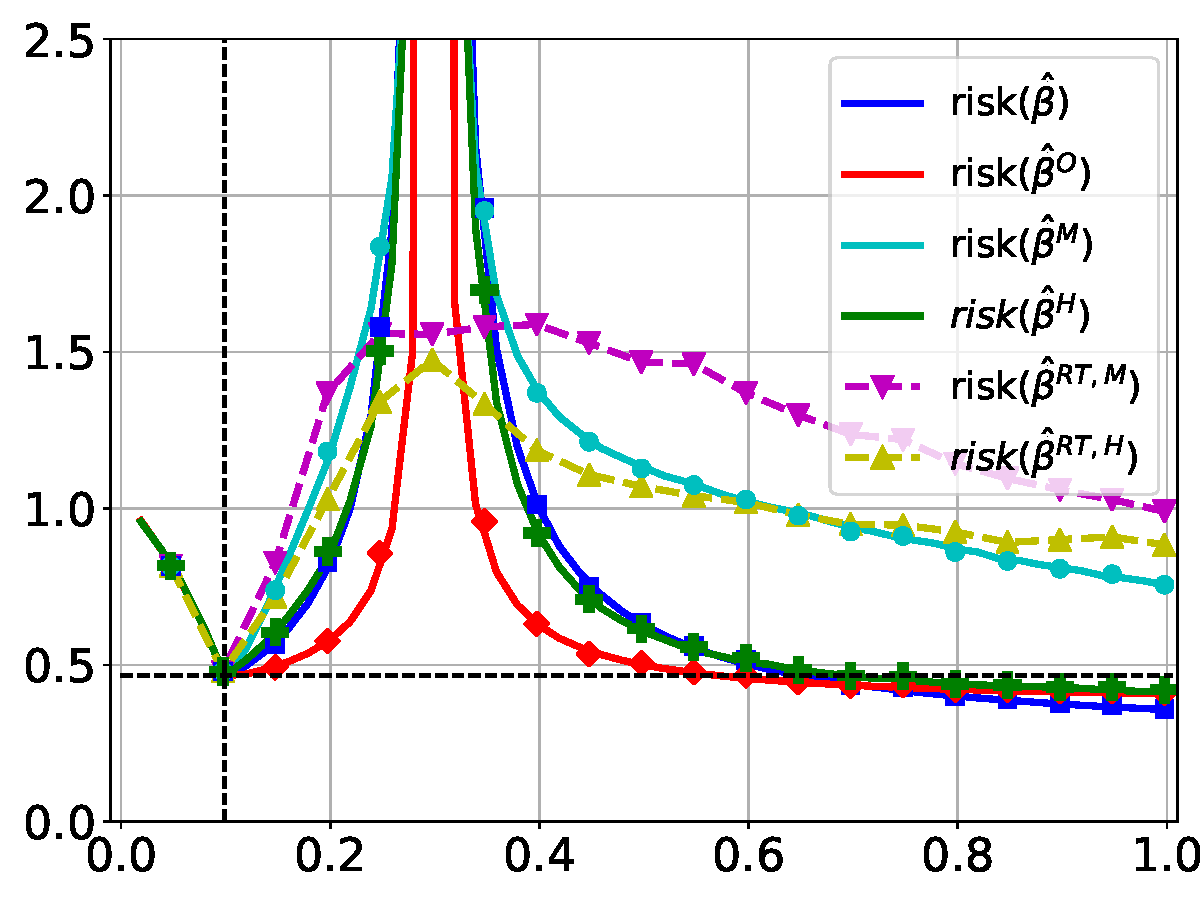
\includegraphics[scale=0.33]{figs/SPIKE_SIM_RT_s10_n30_p100_SCL25}};
	%\node at (-2.4,0) [rotate=90,scale=1.]{Test Risk};
		\node at (-3.5,0) [rotate=90,scale=.9]{Test Risk};
	\node at (0,-2.8) [scale=.9]{Problem Size ($k/p$)};%Each bar in the figure shows the correlations' geometric mean of datasets in this group when training to corresponding non-zero level. 
	\end{tikzpicture}\caption{\small{Spiked covariance, identical latent weights.}}\label{figSM1b}\vspace{-0.2cm}
\end{subfigure}\caption{\small{Same as Figure \ref{fig1} however retraining curves are included. Our asymptotic prediction for various pruning strategies in linear gaussian models with $s/p=0.1$ and $n/p=0.3$. We solve ERM using the first $k$ features and then prune to obtain an $s$-sparse model. The vertical dashed line shows the $k=s$ point. The horizontal dashed line highlights the minimum risk among all underparameterized solutions including retraining. Retraining curves are not displayed.}}\label{figSM1}\vspace{-15pt}
\end{figure}


%\subsection{Further Intuitions: Denoising affect of overparameterization}
%To provide further insights into the pruning benefits of overparameterization, consider a simple linear model with noise level $\sigma=0$, $n\geq p\gg s$ and identity covariance. Pick index set $\Delta\subset[p]$ with $|\Delta|=s$. Suppose we wish to estimate the coefficients $\bt^\st_{\Delta}$. For pruning, we can pick $\Delta$ to be the most salient/largest entries. If we solve the smaller problem over $\Delta$, $\bth(\Delta)$ will only provide a noisy estimate of $\bt^\st_{\Delta}$. The reason is that, the signal energy of missing features $[p]-\Delta$ act as noise uncorrelated with features in $\Delta$. Conversely, if we solve ERM with all features (the larger problem), we perfectly recover  $\bt^\st$ due to lack of noise and $n>p$ from which we perfectly estimate $\bt^\st_{\Delta}$. This simple argument, which is partly inspired by the missing feature setup in \cite{hastie2019surprises}, shows that solving the larger problem with more parameters can have a ``denoising-like effect" and perform better than the small problem. It also explains why retraining again with few features can potentially hurt the performance. This is because when features are uncorrelated (e.g.~diagonal covariance), missing features (due to the smaller problem size) act like additive uncorrelated noise. Our contribution obviously goes well beyond this discussion and theoretically characterizes exact asymptotics, addresses a general covariance model, and highlights the importance of the  overparameterized regime $n\ll p$.
